% gc-13-AreaVolume.tex

\documentclass[xcolor=dvipsnames]{beamer}
\usepackage{teachbeamer}
\title{Area and Volume}
\subtitle{{\CourseNumber}, BCIT}

\author{\CourseName}

\date{March 21, 2018}

\begin{document}

\begin{frame}
  \titlepage
\end{frame}

\begin{frame}
  \frametitle{Negative Area I}
Consider the following problem.
\begin{block}{}
Find the area under the curve $y=x^{2}-4$ between $x=1$ and $x=3$.
\end{block}
\begin{figure}[h]
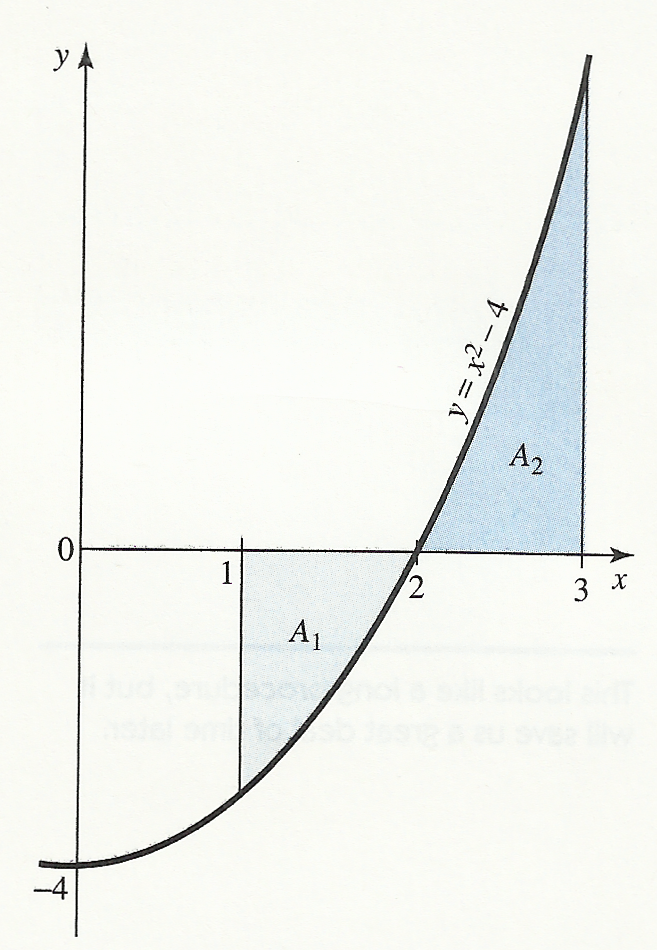
\includegraphics[scale=.6]{./diagrams/negarea.png}
\end{figure}
\end{frame}

\begin{frame}
  \frametitle{Negative Area II}
To solve this problem, find the $x$-intercept and treat the positive
and negative area separately. 
\begin{equation}
  \label{eq:aisohphu}
  \vert{}A_{1}\vert{}+\vert{}A_{2}\vert{}=-\int_{1}^{2}(x^{2}-4)\,dx+\int_{1}^{2}(x^{2}-4)\,dx=-\left(-\frac{5}{3}\right)+\frac{7}{3}=4\notag
\end{equation}
\end{frame}

\begin{frame}
  \frametitle{Negative Area Exercise}
  Find the area between the curve $y=2(x-5)^{2}-2$ and the $x$-axis
  between $x=3$ and $x=7$.
\begin{figure}[h]
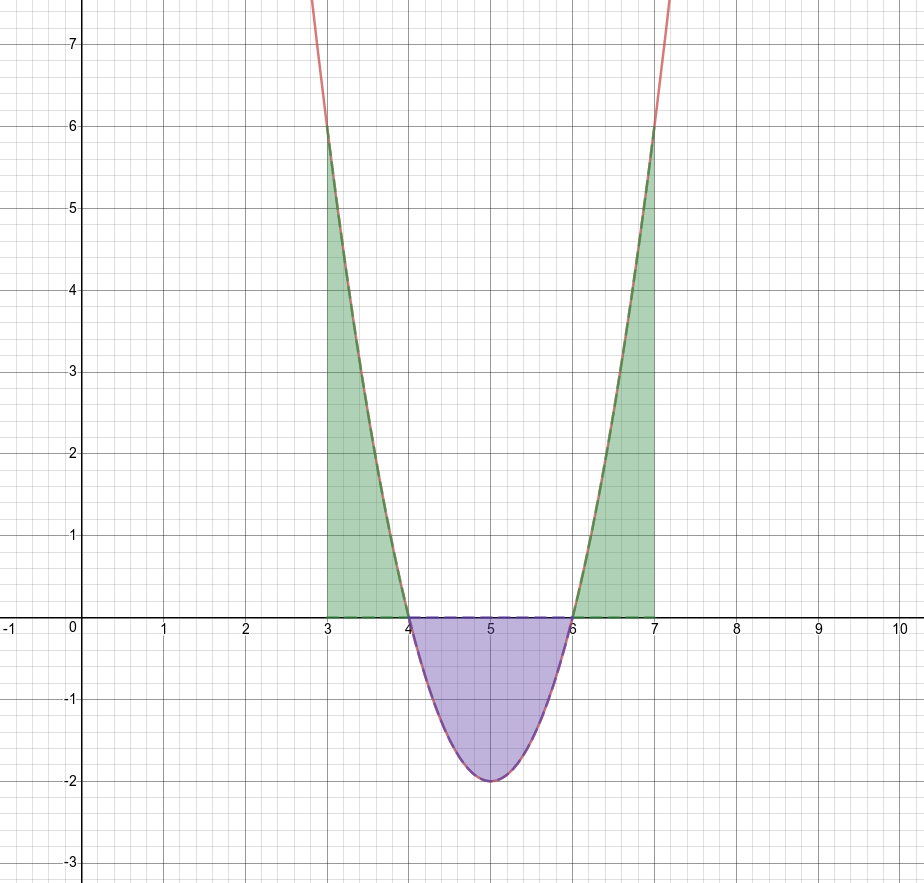
\includegraphics[scale=.2]{./diagrams/NegativeArea.png}
\end{figure}
\end{frame}

\begin{frame}
  \frametitle{Area Between Curves}
  Find the area bounded by the curves $f(x)$ and $g(x)$.
\begin{figure}[h]
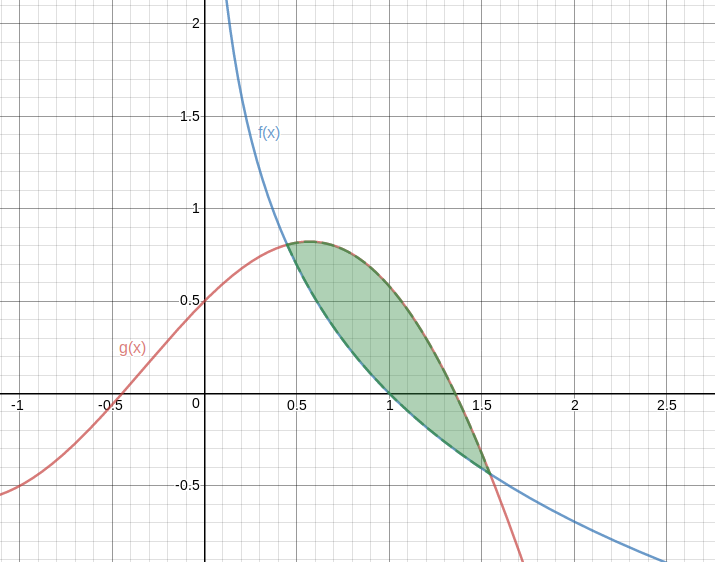
\includegraphics[scale=.15]{./diagrams/areabetwcurs.png}
\end{figure}
To find this area, solve for the two solutions $x_{1},x_{2}$ of 
\begin{equation}
  \label{eq:aikooyae}
  f(x)=g(x)
\end{equation}
(you may have to use Newton's method) and then integrate
\begin{equation}
  \label{eq:upofahma}
  A=\int_{x_{1}}^{x_{2}}\left(g(x)-f(x)\right)\,dx
\end{equation}
\end{frame}

\begin{frame}
  \frametitle{Area Between Curves Exercise}
{\ubung} Find the area of the region enclosed by the parabola
$y=2-x^{2}$ and the line $y=-x$. 
\begin{figure}[h]
  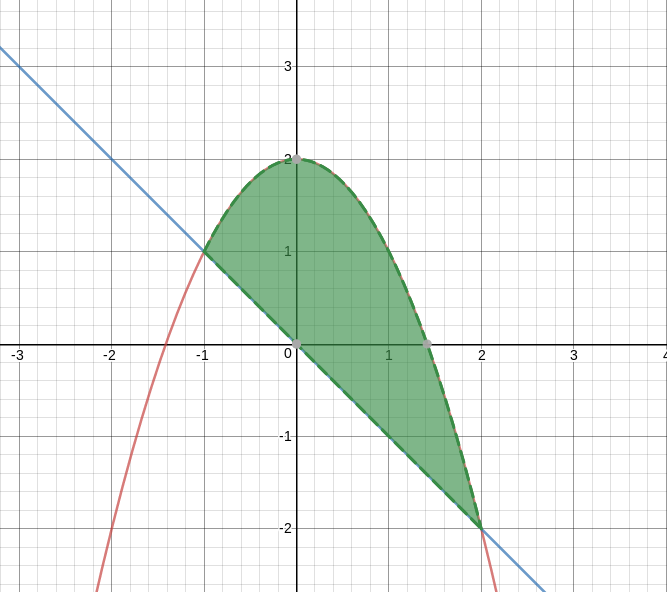
\includegraphics[scale=0.2]{./diagrams/areabc.png}
\end{figure}
\end{frame}

\begin{frame}
  \frametitle{Integrating Along the $y$-Axis}
  Find the area bounded by the curves $y^{2}=12x$ and $y^{2}=24x-36$.
\begin{figure}[h]
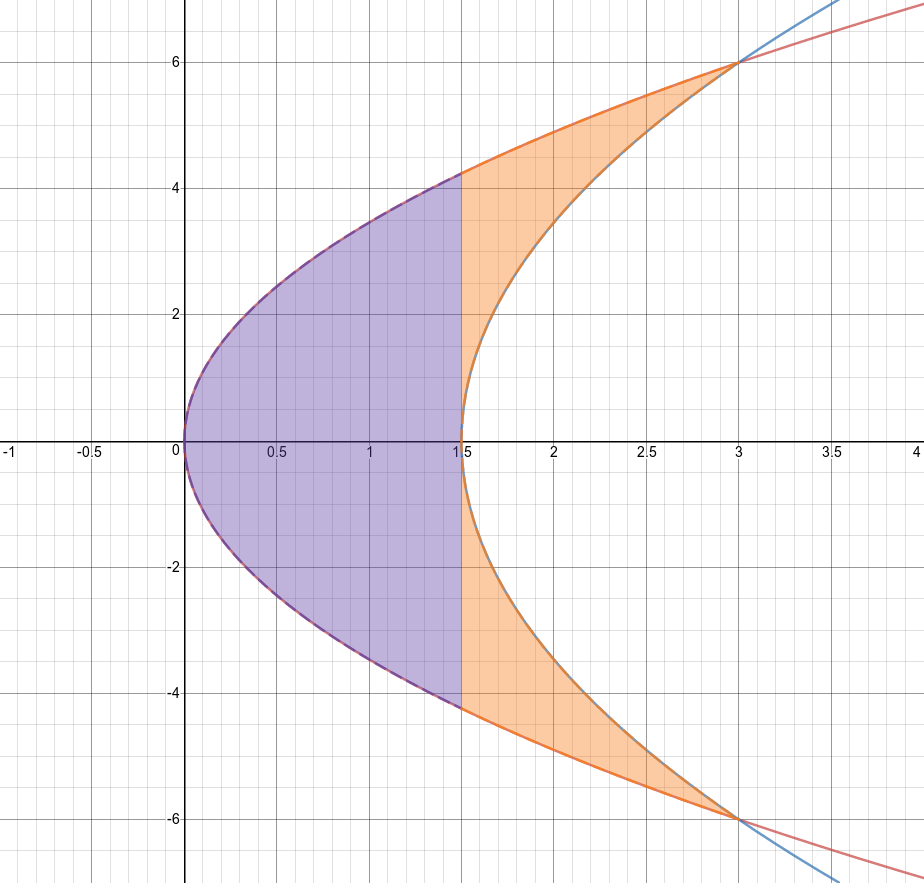
\includegraphics[scale=.15]{./diagrams/AreaBetweenTwoCurves.png}
\end{figure}
In this case, it is more efficient to integrate over $y$.
\begin{equation}
  \label{eq:nuabianu}
  A=2\cdot\int_{0}^{6}\left(\frac{y^{2}}{24}+\frac{36}{24}-\frac{y^{2}}{12}\right)\,dy
\end{equation}
\end{frame}

\begin{frame}
  \frametitle{Area Between Curves Exercise}
  {\ubung} The area of the region that lies to the right of the
  $y$-axis and to the left of the parabola $x=2y-y^{2}$ (the shaded
  region in the figure) is given by the integral 
  \begin{equation}
    \label{eq:ooghoosh}
    \int_{0}^{2}(2y-y^{2})\,dy
  \end{equation}
  Find the area of the region.
  \begin{figure}[h]
    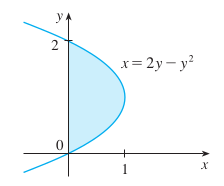
\includegraphics[scale=0.5]{./diagrams/areacurves.png}
  \end{figure}
\end{frame}

\begin{frame}
  \frametitle{Finding an Area Example}
  {\ubung} The figure shows a region consisting of all points inside a
  square that are closer to the center than to the sides of the
  square. Find the area of the region.
  \begin{figure}[h]
    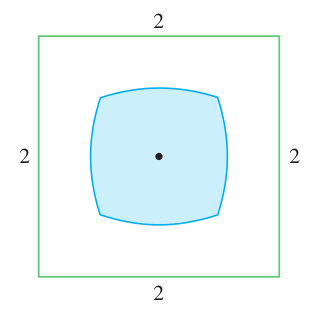
\includegraphics[scale=0.5]{./diagrams/squarish.png}
  \end{figure}
\end{frame}

\begin{frame}
  \frametitle{Finding an Area Solution}
First, notice that the area $A$ equals
\begin{equation}
  \label{eq:aeghieyu}
  A=(2w)^{2}+8\int_{0}^{w}[g(x)-f(x)]\,dx
\end{equation}
where $w$ is the $x$-coordinate of the top right point on the blue
figure; $f(x)=w$ and $g(x)$ is the function going along the top of the
blue figure. Since
\begin{equation}
  \label{eq:seephoes}
  1-w=\frac{1}{\sqrt{2}}
\end{equation}
it follows that
\begin{equation}
  \label{eq:weipeewi}
  w=1-\frac{1}{\sqrt{2}}
\end{equation}
and
\begin{equation}
  \label{eq:kehuichu}
  g(x)=\frac{1-x^{2}}{2}
\end{equation}
This appears to be incorrect.
\end{frame}

\begin{frame}
  \frametitle{Volume of Cross-Sections}
  The volume of a solid integrable cross-sectional area $A(x)$ from
  $x=a$ to $x=b$ is the integral of $A$ from $a$ to $b$,
  \begin{equation}
    \label{eq:upiecait}
    V=\int_{a}^{b}A(x)\,dx
  \end{equation}
  \begin{figure}[h]
    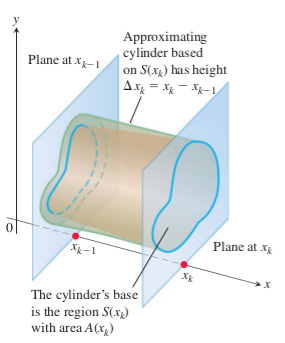
\includegraphics[scale=0.45]{./diagrams/crosssec.png}
  \end{figure}
\end{frame}

\begin{frame}
  \frametitle{Volume of Cross-Sections Exercise}
{\ubung} A pyramid three metres high has a square base that is 3
metres on a side. The cross-section of the pyramid perpendicular to
the altitude $x$ metres down from the vertex is a square, whose side is
$x$ metres. Find the volume of the pyramid.
\begin{figure}[h]
  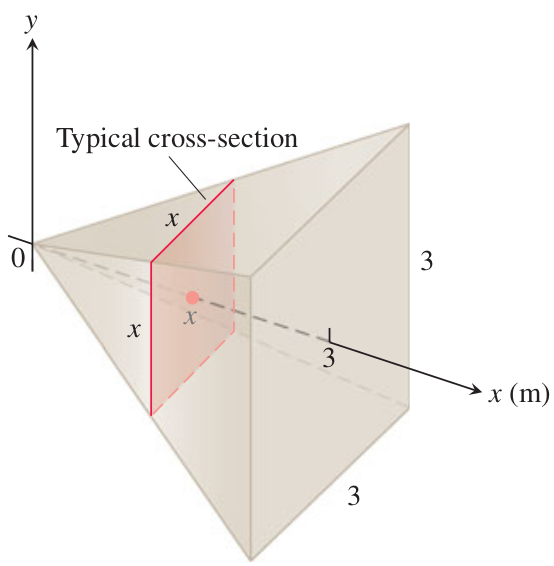
\includegraphics[scale=0.3]{./diagrams/pyramidvol.png}
\end{figure}
\end{frame}

\begin{frame}
  \frametitle{Cavalieri's Principle}
  \begin{block}{Cavalieri's Principle}
    Suppose two regions in three-dimensional space (solids) are
    included between two parallel planes. If every plane parallel to
    these two planes intersects both regions in cross-sections of
    equal area, then the two regions have equal volumes.
  \end{block}
  \begin{figure}[h]
    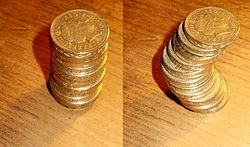
\includegraphics[scale=2]{./diagrams/cavalieri.jpg}
  \end{figure}
\end{frame}

% \textcolor{white}{Here is some invisible stuff.}

\begin{frame}
  \frametitle{Disk Method}
Remember the formula for the volume of a cone:
\begin{equation}
  \label{eq:veishiir}
   V=\frac{1}{3}r^{2}\pi{}h 
\end{equation}

Let's see if we can give a reason for the formula using calculus. Let
the height of a cone be $h$ and the radius $r$.

\begin{figure}[h]
  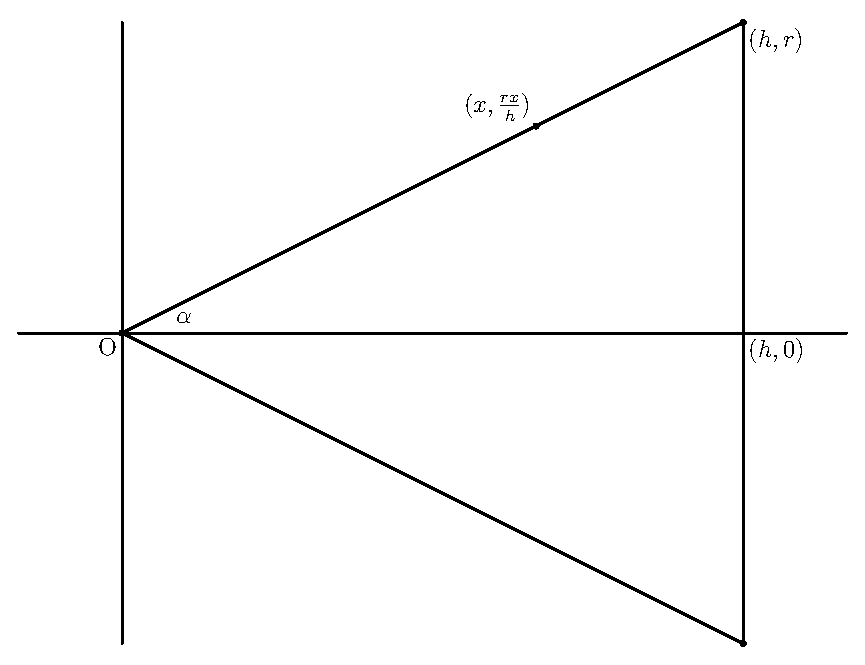
\includegraphics[scale=0.4]{./diagrams/conevol.eps}
\end{figure}
\end{frame}

\begin{frame}
  \frametitle{Disk Method}
  Using the volume of cross-sections formula,
\begin{equation}
  \label{eq:deiwizou}
  A(x)=\left(\frac{rx}{h}\right)^{2}\cdot\pi
\end{equation}
and therefore
\begin{equation}
  \label{eq:eebeoghe}
  V=\int_{0}^{h}A(x)\,dx=\left[\frac{r^{2}\pi{}x^{3}}{3h^{2}}\right]_{0}^{h}=\frac{1}{3}r^{2}\pi{}h
\end{equation}
More generally, any integrable function rotated around the $x$-axis gives us the
volume of a solid by the so-called \alert{disk method} (see the
diagram on the next slide),
\begin{equation}
  \label{eq:eipahbuy}
  V=\int_{a}^{b}\pi[R(x)]^{2}\,dx
\end{equation}
\end{frame}

\begin{frame}
  \frametitle{Disk Method Exercise}
{\ubung} The region between the curve $y=\sqrt{x}$, $0\leq{}x\leq{}4$,
and the $x$-axis is revolved about the $x$-axis to generate a solid.
Find its volume.
  \begin{figure}[h]
    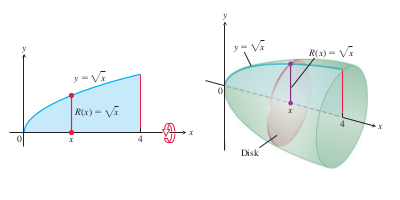
\includegraphics[scale=0.65]{./diagrams/disk_ed.png}
  \end{figure}
\end{frame}

\begin{frame}
  \frametitle{Disk Method Exercise}
{\ubung} The circle
\begin{equation}
  \label{eq:ohtooquu}
  x^{2}+y^{2}=r^{2}
\end{equation}
is rotated about the $x$-axis to generate a sphere. Find its volume.
\begin{figure}[h]
  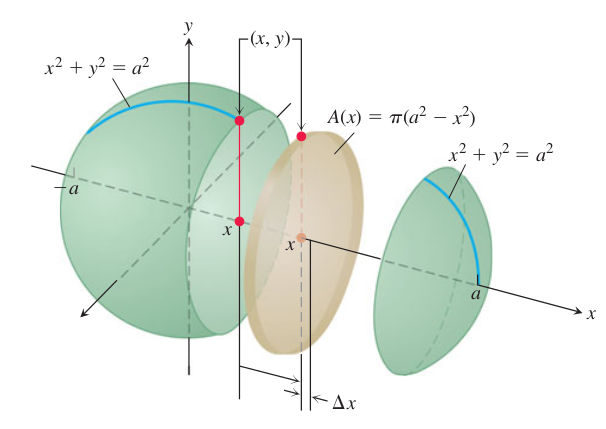
\includegraphics[scale=0.4]{./diagrams/spherevol.png}
\end{figure}
\end{frame}

\begin{frame}
  \frametitle{Disk Method Exercise}
{\ubung} Find the volume of the solid generated by revolving the
region between the parabola 
\begin{equation}
  \label{eq:raejibei}
  x=y^{2}+1
\end{equation}
and the line $x=3$ about the line $x=3$. \textcolor{white}{The solution is $(1/15)\cdot{}64\pi\sqrt{2}$.}
\begin{figure}[h]
  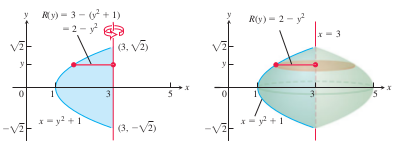
\includegraphics[scale=0.7]{./diagrams/revthr.png}
\end{figure}
\end{frame}

\addtocounter{exercise}{-1}
\addtocounter{equation}{-1}

\begin{frame}
  \frametitle{Disk Method Exercise}
{\ubung} Find the volume of the solid generated by revolving the
region between the parabola 
\begin{equation}
  \label{eq:ebaikeiw}
  x=y^{2}+1
\end{equation}
and the line $x=3$ about the line $x=3$. The solution is $(1/15)\cdot{}64\pi\sqrt{2}$.
\begin{figure}[h]
  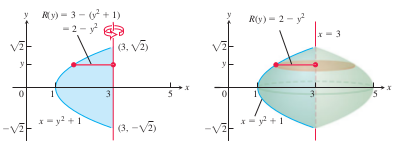
\includegraphics[scale=0.7]{./diagrams/revthr.png}
\end{figure}
% Thomas, page 370, and Schmierbuch, page 2083
\end{frame}

\begin{frame}
  \frametitle{Washer Method Exercise}
{\ubung} The region bounded by the curve $y=x^{2}+1$ and the line
$y=-x+3$ is revolved around the $x$-axis to generate a solid. Find the
volume of the solid.
\begin{figure}[h]
  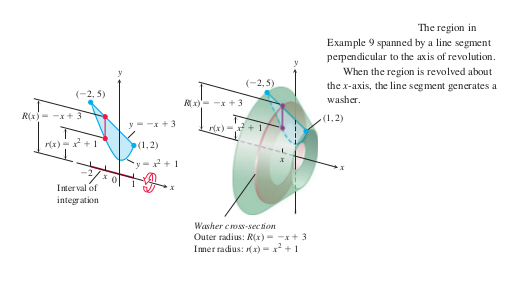
\includegraphics[scale=0.65]{./diagrams/washer.png}
\end{figure}
\end{frame}

\begin{frame}
  \frametitle{Washer Method Exercise}
{\ubung} The region bounded by the parabola $y=x^{2}$ and the line
$y=2x$ in the first quadrant is revolved about the $y$-axis to
generate a solid. Find the volume of the solid.
\begin{figure}[h]
  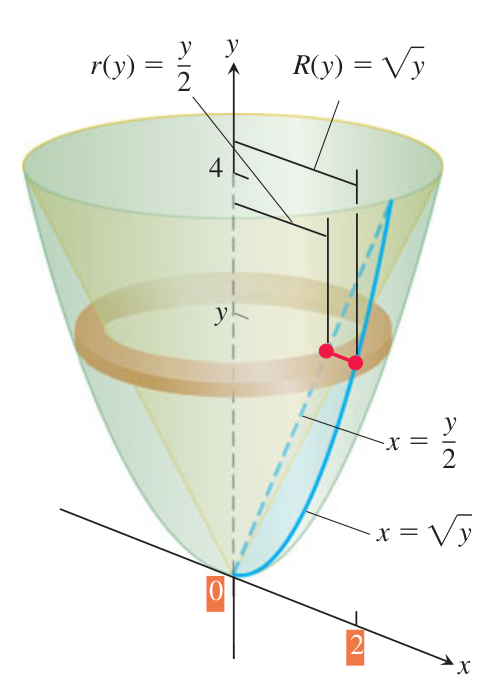
\includegraphics[scale=0.25]{./diagrams/radii.png}
\end{figure}
\end{frame}

\begin{frame}
  \frametitle{Arc Length}
  A curve $y=f(x)$ is called \alert{smooth} on an interval $[a,b]$ if
  $f(x)$ has a continuous derivative at every point of $[a,b]$. The
  length of the polygonal path $P_{0}P_{1}P_{2}\cdots{}P_{n}$
  approximates the length of the curve $y=f(x)$ from point $A$ to
  point $B$.
  \begin{figure}[h]
    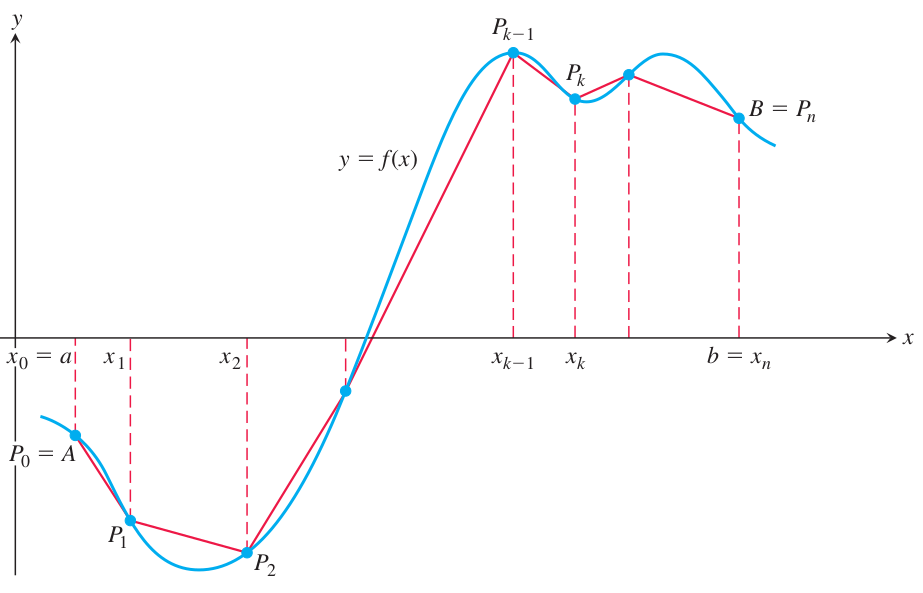
\includegraphics[scale=0.25]{./diagrams/pollen.png}
  \end{figure}
  \end{frame}

\begin{frame}
  \frametitle{Arc Length}
  As we did for the fundamental theorem of calculus, divide up the
  interval $[a,b]$ into intervals of equal length $[x_{i},x_{i+1}]$,
  where $i=0,\ldots,n-1$ and $a=x_{0},b=x_{n}$. Then the length of the
  curve $y=f(x)$ from $a$ to $b$ is
  \begin{equation}
    \label{eq:eeyohpha}
    L=\lim_{n\rightarrow\infty}\sum_{i=0}^{n-1}\sqrt{\left(f(x_{i+1})-f(x_{i})\right)^{2}+\left(x_{i+1}-x_{i}\right)^{2}}
  \end{equation}
The mean value theorem tells us that there is always a point
$x_{i}^{\ast}$ between $x_{i}$ and $x_{i+1}$ such that
\begin{equation}
  \label{eq:oshachie}
  f'(x_{i}^{\ast})=\frac{f(x_{i+1})-f(x_{i})}{x_{i+1}-x_{i}}
\end{equation}
\end{frame}

\begin{frame}
  \frametitle{Arc Length}
Consequently,
  \begin{equation}
    \label{eq:ahchoode}
    L=\lim_{n\rightarrow\infty}\sum_{i=0}^{n-1}\sqrt{\left(f'(x_{i}^{\ast})\left(x_{i+1}-x_{i}\right)\right)^{2}+\left(x_{i+1}-x_{i}\right)^{2}}
  \end{equation}
which is equivalent to
\begin{equation}
  \label{eq:jooquaiw}
    L=\lim_{n\rightarrow\infty}\sum_{i=0}^{n-1}\left(x_{i+1}-x_{i}\right)\sqrt{\left(1+f'(x_{i}^{\ast})\right)^{2}}
\end{equation}
Now let $g$ be the function
\begin{equation}
  \label{eq:eicahdei}
  g(x)=\sqrt{1+\left(f'(x)\right)^{2}}
\end{equation}
\end{frame}

\begin{frame}
  \frametitle{Arc Length}
Then
\begin{equation}
  \label{eq:geiphofi}
    L=\lim_{n\rightarrow\infty}\sum_{i=0}^{n-1}\left(x_{i+1}-x_{i}\right)g(x_{i}^{\ast})
\end{equation}
We already know from the fundamental theorem of calculus that this is
\begin{equation}
  \label{eq:yemaezov}
    L=\int_{a}^{b}g(x)\,dx=\int_{a}^{b}\sqrt{1+\left(f'(x)\right)^{2}}\,dx
\end{equation}
This is our \alert{formula for arc length}.
\end{frame}

\begin{frame}
  \frametitle{Arc Length Exercise}
{\ubung} Find the length of the curve
  \begin{equation}
    \label{eq:ahwushei}
    y=\frac{4\sqrt{2}}{3}x^{\frac{3}{2}}-1,0\leq{}x\leq{}1
  \end{equation}
Check the plausibility of your result by approximating the curve
length calculating the straight-line distance between the two end
points.
\end{frame}

\begin{frame}
  \frametitle{Arc Length Exercise}
{\ubung} Find the length of the curve
  \begin{equation}
    \label{eq:aecejaej}
    y=\frac{x^{3}}{12}+\frac{1}{x},1\leq{}x\leq{}4
  \end{equation}
Check the plausibility of your result by approximating the curve
length calculating the straight-line distance between the two end
points.
\end{frame}

\begin{frame}
  \frametitle{Arc Length Exercise}
{\ubung} A telephone line hangs between two poles 14 metres apart in
the shape of a catenary
\begin{equation}
  \label{eq:lufaebeg}
  y=20\cosh\left(\frac{x}{20}\right)-15
\end{equation}
where $x$ and $y$ are measured in metres. Find the length of telephone
wire needed between the two poles. \textcolor{white}{The answer is $20(\sinh(7/20)-\sinh(-7/20))=14.288$.}
\begin{figure}[h]
  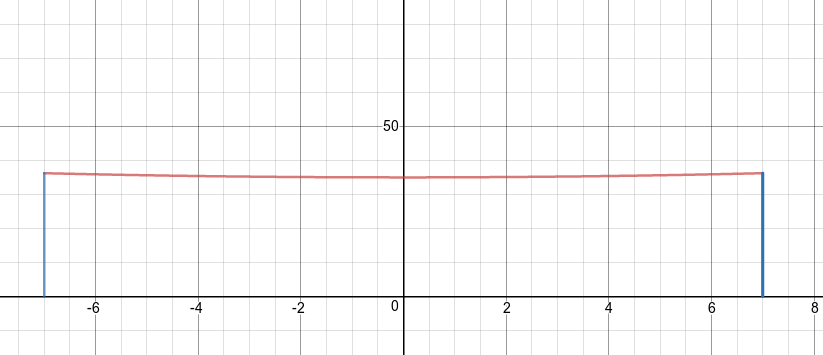
\includegraphics[scale=0.22]{./diagrams/telwire.png}
\end{figure}
\end{frame}

\addtocounter{equation}{-1}
\addtocounter{exercise}{-1}

\begin{frame}
  \frametitle{Arc Length Exercise}
{\ubung} A telephone line hangs between two poles 14 metres apart in
the shape of a catenary
\begin{equation}
  \label{eq:aeweerae}
  y=20\cosh\left(\frac{x}{20}\right)-15
\end{equation}
where $x$ and $y$ are measured in metres. Find the length of telephone
wire needed between the two poles. The answer is $20(\sinh(7/20)-\sinh(-7/20))=14.288$.
\begin{figure}[h]
  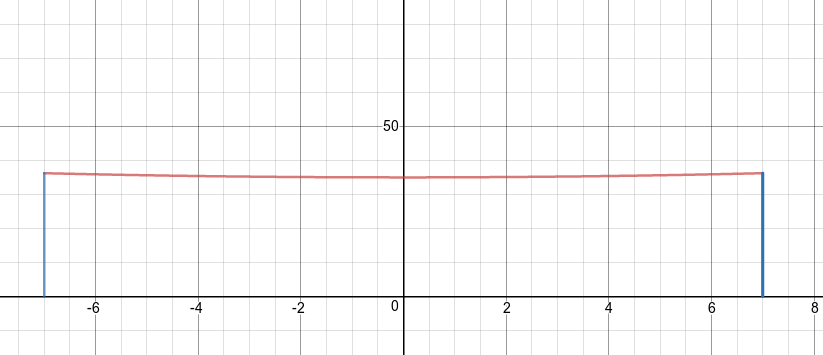
\includegraphics[scale=0.22]{./diagrams/telwire.png}
\end{figure}
\end{frame}

\begin{frame}
  \frametitle{Surface Area}
  If the function $f(x)\geq{}0$ is continuously differentiable on
  $[a,b]$, the \alert{area of the surface} generated by revolving the
  graph of $y=f(x)$ about the $x$-axis is
  \begin{equation}
    \label{eq:xaimosah}
    S=\int_{a}^{b}2\pi{}f(x)\sqrt{1+\left(f'(x)\right)^{2}}\,dx
  \end{equation}
\end{frame}

\begin{frame}
  \frametitle{Surface Area Exercise}
{\ubung}  Show that the lateral surface area of a frustum (without base and top) is
\begin{equation}
  \label{eq:eequochi}
  S=2\pi{}y^{\ast}L
\end{equation}
where $y^{\ast}$ is the average height of $AB$ above the $x$-axis and
$L$ is the length of $AB$.
\begin{figure}[h]
  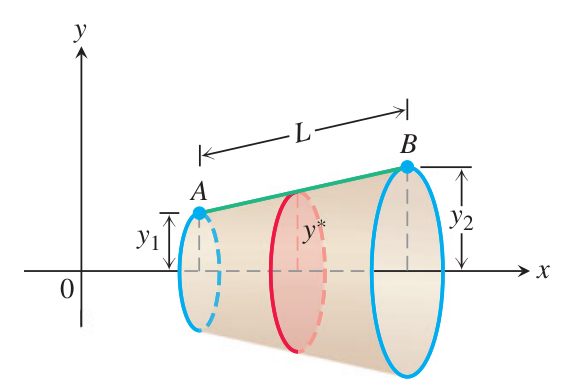
\includegraphics[scale=0.3]{./diagrams/frustumarea.png}
\end{figure}
\end{frame}

\begin{frame}
  \frametitle{Surface Area Exercise}
{\ubung} Find the area of the surface generated by revolving the curve
$y=2\sqrt{x}$, $1\leq{}x\leq{}2$, about the $x$-axis.
\begin{figure}[h]
  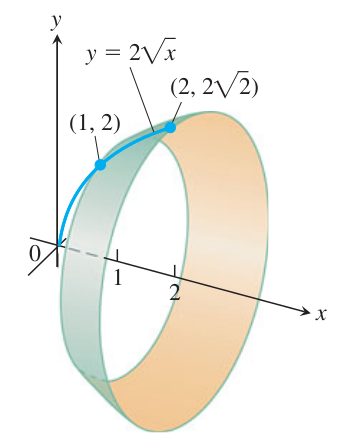
\includegraphics[scale=0.3]{./diagrams/revosurf1.png}
\end{figure}
\addtocounter{exercise}{-1}
\end{frame}

\begin{frame}
  \frametitle{Surface Area Exercise} 
  {\ubung} Find the area of the surface generated by revolving the
  curve $y=2\sqrt{x}$, $1\leq{}x\leq{}2$, about the $x$-axis. The
  solution is $(8\pi/3)\cdot{}(\sqrt{27}-\sqrt{8})=19.836$.
\begin{figure}[h]
  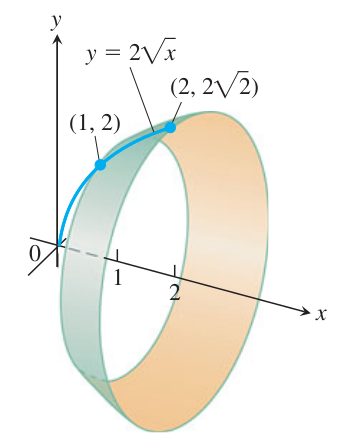
\includegraphics[scale=0.3]{./diagrams/revosurf1.png}
\end{figure}
\end{frame}

\begin{frame}
  \frametitle{Surface Area Exercise}
{\ubung} The line segment $x=1-y,0\leq{}y\leq{}1$, is revolved around
the $y$-axis to generate a cone. Find its lateral surface area (which
excludes the base area).
\begin{figure}[h]
  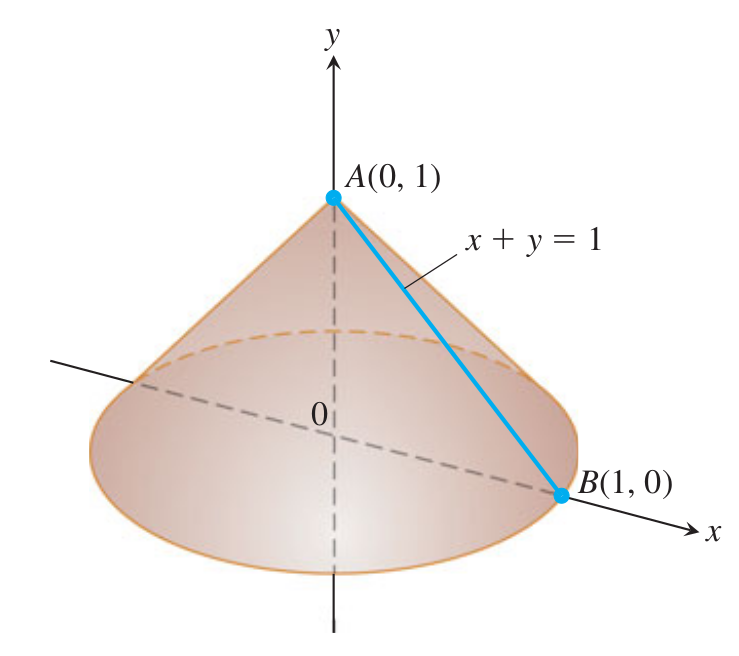
\includegraphics[scale=0.25]{./diagrams/conelateral.png}
\end{figure}
\end{frame}

\begin{frame}
  \frametitle{End of Lesson}
Next Lesson: Integration Methods
\end{frame}

\end{document}

